%!TEX root = ../main.tex
%******************************
%	 Discussion 
%*****************************

\graphicspath{{"../../Dropbox (Cambridge  University)/Figures_for_thesis/Discussion/"}}

\chapter{Conclusion and future directions}  

My work focused on the statistical quantification of transcriptional noise in biological systems such as the activation response of CD4\plus{} T cells. Firstly, in collaboration with Celia P. Martinez-Jimenez, we used scRNA-Seq data of CD4\plus{} T cells to identify an age-related increase in transcriptional noise within a set of immune response genes (see \textbf{Chapter 2}). Assessment of changes in transcriptional variability was restricted to genes that show similar expression levels in naive and active cells or young and old animals. I therefore extended the BASiCS statistical framework to correct for the confounding effect between mean expression $\mu_i$ and over-dispersion $\delta_i$ by introducing a joint prior that captures the dependence of $\delta_i$ on $\mu_i$. The derivation of residual over-dispersion parameters $\epsilon_i$ allowed me to robustly test for changes in expression variability even when genes display changes in mean expression (see \textbf{Chapter 3}). Finally, in collaboration with Christina Ernst, we dissected the transcriptional programme underlying mouse spermatogenesis and characterised developmental processes such as spermatogonia differentiation, meiosis and spermiogenesis. We further identified a set of X-linked, spermatid-specifically expressed genes that show high enrichment of the repressive H3K9me3 mark in their promoter regions. After full characterisation of this differentiation process, I used the extended BASiCS model to identify changes in variability along spermatogenesis.   Abrupt changes in mean expression display a confounding effect when measuring transcriptional variability along this time-course (see \textbf{Chapter 4}).  \\

While recent technological and computational advances of the recent years facilitate the quantification of biological noise across a range of cell types and tissues, major challenges remain regarding robust measurement, mathematical modelling and experimental validation. Here, I discuss the results of my work in light of current challenges in the field of scRNA-Seq when measuring biological variation across individual cells.

\newpage

\section{Technologies to study the biological role of noise}

The results of \textbf{Chapter 2} indicate two different settings where changes in variability are either related to the synchronisation of a dynamic cellular system or the disruption of such a system. We explored the effect of ageing on transcriptional noise during immune activation using scRNA-Seq data. Early immune activation induces a transcriptional switch from stochastic to regulated gene expression coupled with a reduction in transcriptional variability. These dynamics and, more importantly, a set of immune-related response genes are conserved during evolution. While ageing only shows subtle effects on the overall transcriptomic profiles of individual cells, we observe a strong increase in expression variability in the core set of immune response genes during ageing. Therefore, transcriptional variability is a largely unexplored factor of organismal ageing. This finding has been validated by several studies \citep{Enge2017, Angelidis2018, Cheung2018} adding the increase in transcriptional noise to the list of ageing-associated physiological effects.\\

Our study uncovered transcriptional noise as a factor that disturbs the dynamic response of an otherwise tightly regulated system. The systematic analysis of how transcriptional noise globally influences other cellular systems such as the developing embryo or disease onset is still lacking. Examples of studies that identified a link between cell fate commitment and heterogeneous gene expression using scRNA-Seq data include the development of the 4-cell stage embryo towards extraembryonic and pluripotent cell lineages \citep{Goolam2016}. Furthermore, Mohammed \emph{et al.}, 2017 identified global changes in transcriptional noise during early mouse embryo development that correlate with the plasticity of cell populations. Pluripotent cells tend to display noisier gene expression compared to committed cells \citep{Mohammed2017}. Nevertheless, technical limitations restricted the analysis to few hundreds of cells and specific tissues per embryo. With the newly developed combinatorial indexing approaches, hundreds of thousands of transcriptomes can be generated in parallel \citep{Cao2017}. This allows an unbiased detection of all major cell-types during (e.g.) embryonic development, which in turn offers a great resource to perform systematic comparisons of transcriptional noise between tissues and time-points. Major drawbacks of this approach would be the reduced sequencing depth and the inability to validate the global change in variability as discussed below.\\

In \textbf{Section \ref{sec2:droplet}}, I tested for changes in expression variability between the pre-somitic and the somitic mesoderm of the developing mouse embryo. Interestingly, this analysis revealed heterogeneous up-regulation of lineage-associated genes that are later on expressed in defined tissues. This shows that testing for changes in expression variability can lead to the identification of uncharacterised, early commitment processes during embryogenesis. Nevertheless, scRNA-Seq data does not directly allow identification of the underlying transcriptional regulation that induces heterogeneous expression of these genes. It is therefore impossible to predict whether heterogeneity in expression is induced by molecular noise or driven by deterministic processes.\\

So far, quantification of expression noise on a genome wide scale is only possible by scRNA-Seq. This raises the question if noise that is detected on the mRNA level propagates to form fluctuations in proteins which are the final driver for phenotypic variations between individual cells. Reports have been published that show a reduction of transcriptional noise during nuclear export of mRNAs \citep{Battich2015a, BaharHalpern2015a} indicating the possibility that studying biological noise on the mRNA level is further buffered in the cytoplasm by mechanisms such as miRNA-based degradation \citep{Schmiedel2015}. In recent years, technologies have been developed to measure protein abundance in single cells in high-throughput and high-content based approaches. \Gls{CyTOF} has been introduced as a single-cell technology to measure multiple proteins within hundreds of thousands of cells. For this, antibodies against membrane bound and intracellular proteins are labelled with transition element isotopes and quantified via mass spectroscopy. So far, the main application of CyTOF has been to identify immune cell dynamics \citep{Bendall2011}. To add the spatial component to mass cytometry, Giesen \emph{et al.}, 2014 developed imaging mass cytometry to obtain spatial distributions of 32 proteins in breast cancer samples \citep{Giesen2014}. A similar approach has been introduced by Gut \emph{et al.}, 2018 where off-the shelf antibodies are used to spatially resolve protein expression. During 20 rounds of primary and fluorescently-labelled secondary antibody staining, multiplexed read-outs of protein positions can be obtained from individual cells \citep{Gut2018}. The spatial detection of proteins has been extended by simultaneously measuring mRNA transcripts by isotope tagging \cite{Schulz2018}. These approaches allow (i) quantification of protein expression noise, (ii) spatially-resolved inter- and intra-cellular variations of protein abundance and (iii) the assessment of noise propagation from the mRNA to protein level. To further enhance the connection between mRNA and protein noise, and chromatin state and mRNA noise, multi-omics technologies need to advance in precision and scalability.

\newpage

\section{Confounding effects when measuring noise}

We used the BASiCS framework to quantify and compare measures of transcriptional noise in the immune response of CD4\plus{} T cells. By incorporating reads of synthetic RNA spike-in molecules, BASiCS quantifies and removes technical noise from the total transcriptional variation. Throughout this thesis, we used the over-dispersion parameter $\delta_i$ to capture biological variability in expression after removal of unwanted technical variation. Furthermore, to account for experimental designs where cells were captured in multiple replicates, BASiCS scales technical noise batch-specifically  \citep{Vallejos2015BASiCS}. We described a genes' mean expression as an additional factor that confounds testing changes in over-dispersion. Therefore, we extended the BASiCS framework to derive residual over-dispersion estimates that show no correlation to mean expression (see \textbf{Chapter 3}). \\

By applying this model to capture changes in variability over the differentiation time-course of spermatogenesis, I observed that the strength of transcriptional changes over time introduce an additional confounding factor that, so far, has not been accounted for. I will therefore discuss a variety of confounding factors that influence the quantification of transcriptional noise, grouping these into experimental and technical effects.

\subsection{Experimental confounding factors}

Transcriptional noise as defined in \textbf{Box 1} can only be measured in truly homogeneous populations of cells. Previous studies that quantified transcriptional variability from scRNA-Seq data either sequenced mESCs (e.g.~\citep{Kolodziejczyk2015cell}), primary chicken erythroid progenitor cells \citep{Richard2016}, a murine multipotent hematopoietic precursor cell line \citep{Mojtahedi2016} or CD4\plus T cells \citep{Martinez-jimenez2017}, all of which reside in a homogeneous ground state prior to activation/differentiation. With the development of technologies that capture thousands of cells in an unbiased way, structured heterogeneity presents the major source of cell-to-cell variation in expression. As shown in \textbf{Section \ref{sec2:droplet}}, one relies on clustering approaches to identify homogeneous populations of cells that can be compared when testing for changes in transcriptional variability. It is therefore also crucial to understand the underlying biology that causes structured heterogeneity to avoid including low quality cells in the analysis. For example, Ibarra-Soria \emph{et al.}, 2018 identified a small intermediate population between pre-somitic and somitic mesoderm with unknown identity \citep{Ibarra-Soria2018}. It is recommended to remove such cells from analysis to avoid any unknown biological heterogeneity that confounds biological noise.

\newpage
 
As shown in \textbf{Section \ref{variability_over_PT}}, quantification of transcriptional noise is also heavily influenced by the underlying differentiation programmes of otherwise homogeneous cell populations, as exemplified by the differentiation process of spermatogenesis. After extensive quality control and clustering, the remaining variation in germ cell populations is dictated by genes that strongly and abruptly change their expression levels (e.g.~\textit{Prm1}). This observation is in line with previous reports on how the cell-cycle state of each cell masks underlying population structure \citep{Buettner2015}. For each gene $i$, the \gls{scLVM} captures (e.g.) the cell cycle associated component $\hat{y}_i$ and allows the derivation of corrected counts $y^{\ast}$ by substracting this effect from the observed count $y_i$: $y^{\ast}=y_i-\hat{y}_i$. This correction can therefore be seen as a regression approach to correct for a specific confounding effect (e.g.~cell cycle). To incorporate this idea into the BASiCS framework, it is possible to introduce a flexible regression that accounts for any given confounding effect. In addition to correcting the mean expression effect, the model can be extended to perform a semi-parametric regression between the over-dispersion parameter and a measure of association to differentiation. This measure in the simplest case can be parameters of a regression fit between each cells' expression level and the ordering of cells along the differentiation time-course. 

\subsection{Technical confounding factors}

ScRNA-Seq is prone to high technical noise due to the low starting amounts of RNA transcripts that are first captured, reverse transcribed, pre-amplified, prepared for sequencing and sequenced. Only around 10\%-20\% of all transcripts are captured in each individual cell leading to high levels of technical noise. Furthermore, amplification biases exponentially enhance noise introduced by variation in capture efficiency. These biases are minimized by the introduction of \glspl{UMI} that allow the direct quantification of transcript abundance \cite{Islam2014}. In preliminary analyses to study parameter robustness as displayed in \textbf{Section \ref{sec2:parameter_stabilization}}, we observed that UMI data \citep{Zeisel2015} resulted in generally more robust estimates compared to non-UMI data (e.g.~CD4\plus T cells, \citep{Martinez-jimenez2017}).\\

The incorporation of UMIs into droplet-based scRNA-Seq technologies facilitates a robust estimation of transcriptional variability. On the other hand, these high-throughput methods come at the price of reduced sequencing depth, the inability to quantify technical noise via RNA spike-ins and often reduced replication. A recent study addressed the question of how to allocate a given sequencing budget to scRNA-Seq experiments \citep{Zhang2018}. One can either choose to sequence more cells at lower depth or to  deeply sequence few cells. More reads in fewer cells reduce technical noise when estimating the cellular transcription state while more cells capture the full variance observed in the cell population. The authors propose that the optimal trade-off between number off cells and sequencing depth considering a fixed sequencing budget is an average $\sim$1 UMI per cell detected for the biologically relevant genes \citep{Zhang2018}. This trade-off was found by simulations and sub-sampling experiment similar to the ones displayed in \textbf{Chapter 3}. Further to the results of Zhang \emph{et al.}, 2018, replications of droplet-based scRNA-Seq experiments are important to robustly quantify and validate measures of transcriptional variability. 

\section{Experimental validation and manipulation of noise}

While the results throughout this thesis indicated the functional role of transcriptional variability in dynamic biological systems, one of the main experimental challenges is to alter transcriptional noise to validate the hypothesised role. Classically, unicellular systems were employed to study the sources of transcriptional noise. In these systems, genetic alterations allowed the modulation of transcriptional and translational variability \cite{Raser2004, Raser2005, Ozbudak2002, Hornung2012}. Specifically, changing promoter architecture strongly alters expression noise \cite{Jones2014, Sharon2014}. These simple approaches are not feasible in multicellular organisms, for example, to alter transcriptional noise during embryogenesis. While several regulatory factors on the genomic, epigenetic, transcriptional and translational level influence transcriptional noise, it is difficult to introduce a targeted alteration of certain regulatory factors while simultaneously avoiding down-stream effects other than alterations of transcriptional noise of one or few genes. Dueck \emph{et al.}, 2016 proposed \emph{in vitro} experimental designs to perturb expression variability in cellular systems. Generally, these approaches can be grouped into targeted and general perturbations of transcriptional noise \citep{Dueck2016}.

\subsection{General perturbation of transcriptional noise} 

Dueck \emph{et al.}, 2016 introduced the concept of increasing global transcriptional noise by utilizing the off-target effects of \glspl{siRNA}. Similar to miRNAs, siRNAs are designed to complementarly bind target RNAs and induce their degradation. While most siRNAs lead to the cleavage of cognate RNA, due to partial complementary sequences in off-target RNAs, levels of off-target proteins are also perturbed \citep{Scacheri2004}. By designing a system where siRNAs with primarily off-target effects are expressed under a regulated promoter such as the tetracycline-controlled transcriptional activation system \citep{Gossen1995}, global changes in transcriptional variability can be induced \citep{Dueck2016}. In a similar fashion, the controlled expression of a CRISPR/Cas9 system containing \glspl{sgRNA} with random targets can introduce random deletions or insertions genome wide and therefore increase transcriptional noise. These settings do not control for changes in cellular states due to spontaneous up-or down-regulation of key regulatory components. 

\subsection{Targeted perturbation of transcriptional noise} 

To alter the variation in transcript abundance for specific RNAs, Dueck \emph{et al.} proposed to (i) transfect a selected set of RNAs into specific cells, (ii) transfect the RNAs encoding specific TFs into cells or to (iii) over-express certain miRNAs that target multiple RNAs \cite{Dueck2016}. The first two approaches only increase RNA abundance for specific genes in specific cells. The third approach offers a more intriguing method to modulate protein abundance at the post-transcriptional level as demonstrated by Schmiedel \emph{et al.}, 2015 and 2017 \cite{Schmiedel2015, Schmiedel2017}. The proposed role of miRNAs to reduce noise levels in protein abundance offers an experimental setting where depletion of certain miRNAs by targeted CRISPR/Cas9 interference could potentially increase noise in a set of miRNA targeted genes. This system could, for example, validate an ageing phenotype in the activation response of CD4\plus{} T cells as presented in \textbf{Chapter 2}. \\

The identification of miRNA-driven modulation of transcriptional noise further opens the question of whether transcriptional noise can be modulated by other factors that affect mRNA stability, possibly by altering one out of more than 100 described RNA modifications \citep{Cantara2011}. For example, miRNAs regulate the \gls{m6A} on RNAs by recruiting the methyltransferase METTL3 which affects the reprogramming of mouse embryonic fibroblasts \citep{Chen2015b}. Inducing alterations in the machinery that deposits or recognises such modifications of the RNA could lead to targeted increase or decrease in transcriptional noise.

\newpage

\section{Future approaches to model scRNA-Seq data}

I introduced BASiCS as a Bayesian framework to quantify transcriptional noise from scRNA-Seq data with the main benefit of propagating statistical uncertainty from the data to down-stream differential variability testing.
With the development of droplet-based scRNA-Seq approaches \citep{Macosko2015, Klein2015} and large-scale microwell techniques \citep{Han2018}, the amount of cells that can be assayed in one experiment scaled from hundreds to hundreds of thousands \citep{Svensson2018}. To learn model parameters of a generative model such as BASiCS across all cells and all genes became computationally challenging when considering a full Bayesian MCMC-based approach. To address this problem, a model framework called \gls{scVI} has been developed that uses stochastic optimization within a variational autoencoder network to approximate posterior distributions of model parameters and latent factors \citep{Lopez2018}. In scVI transcriptomes of each cell are encoded through a non-linear transformation into a low-dimensional latent vector of normal random variables. \\

\begin{wrapfigure}{r}{0.5\textwidth}
\centering    
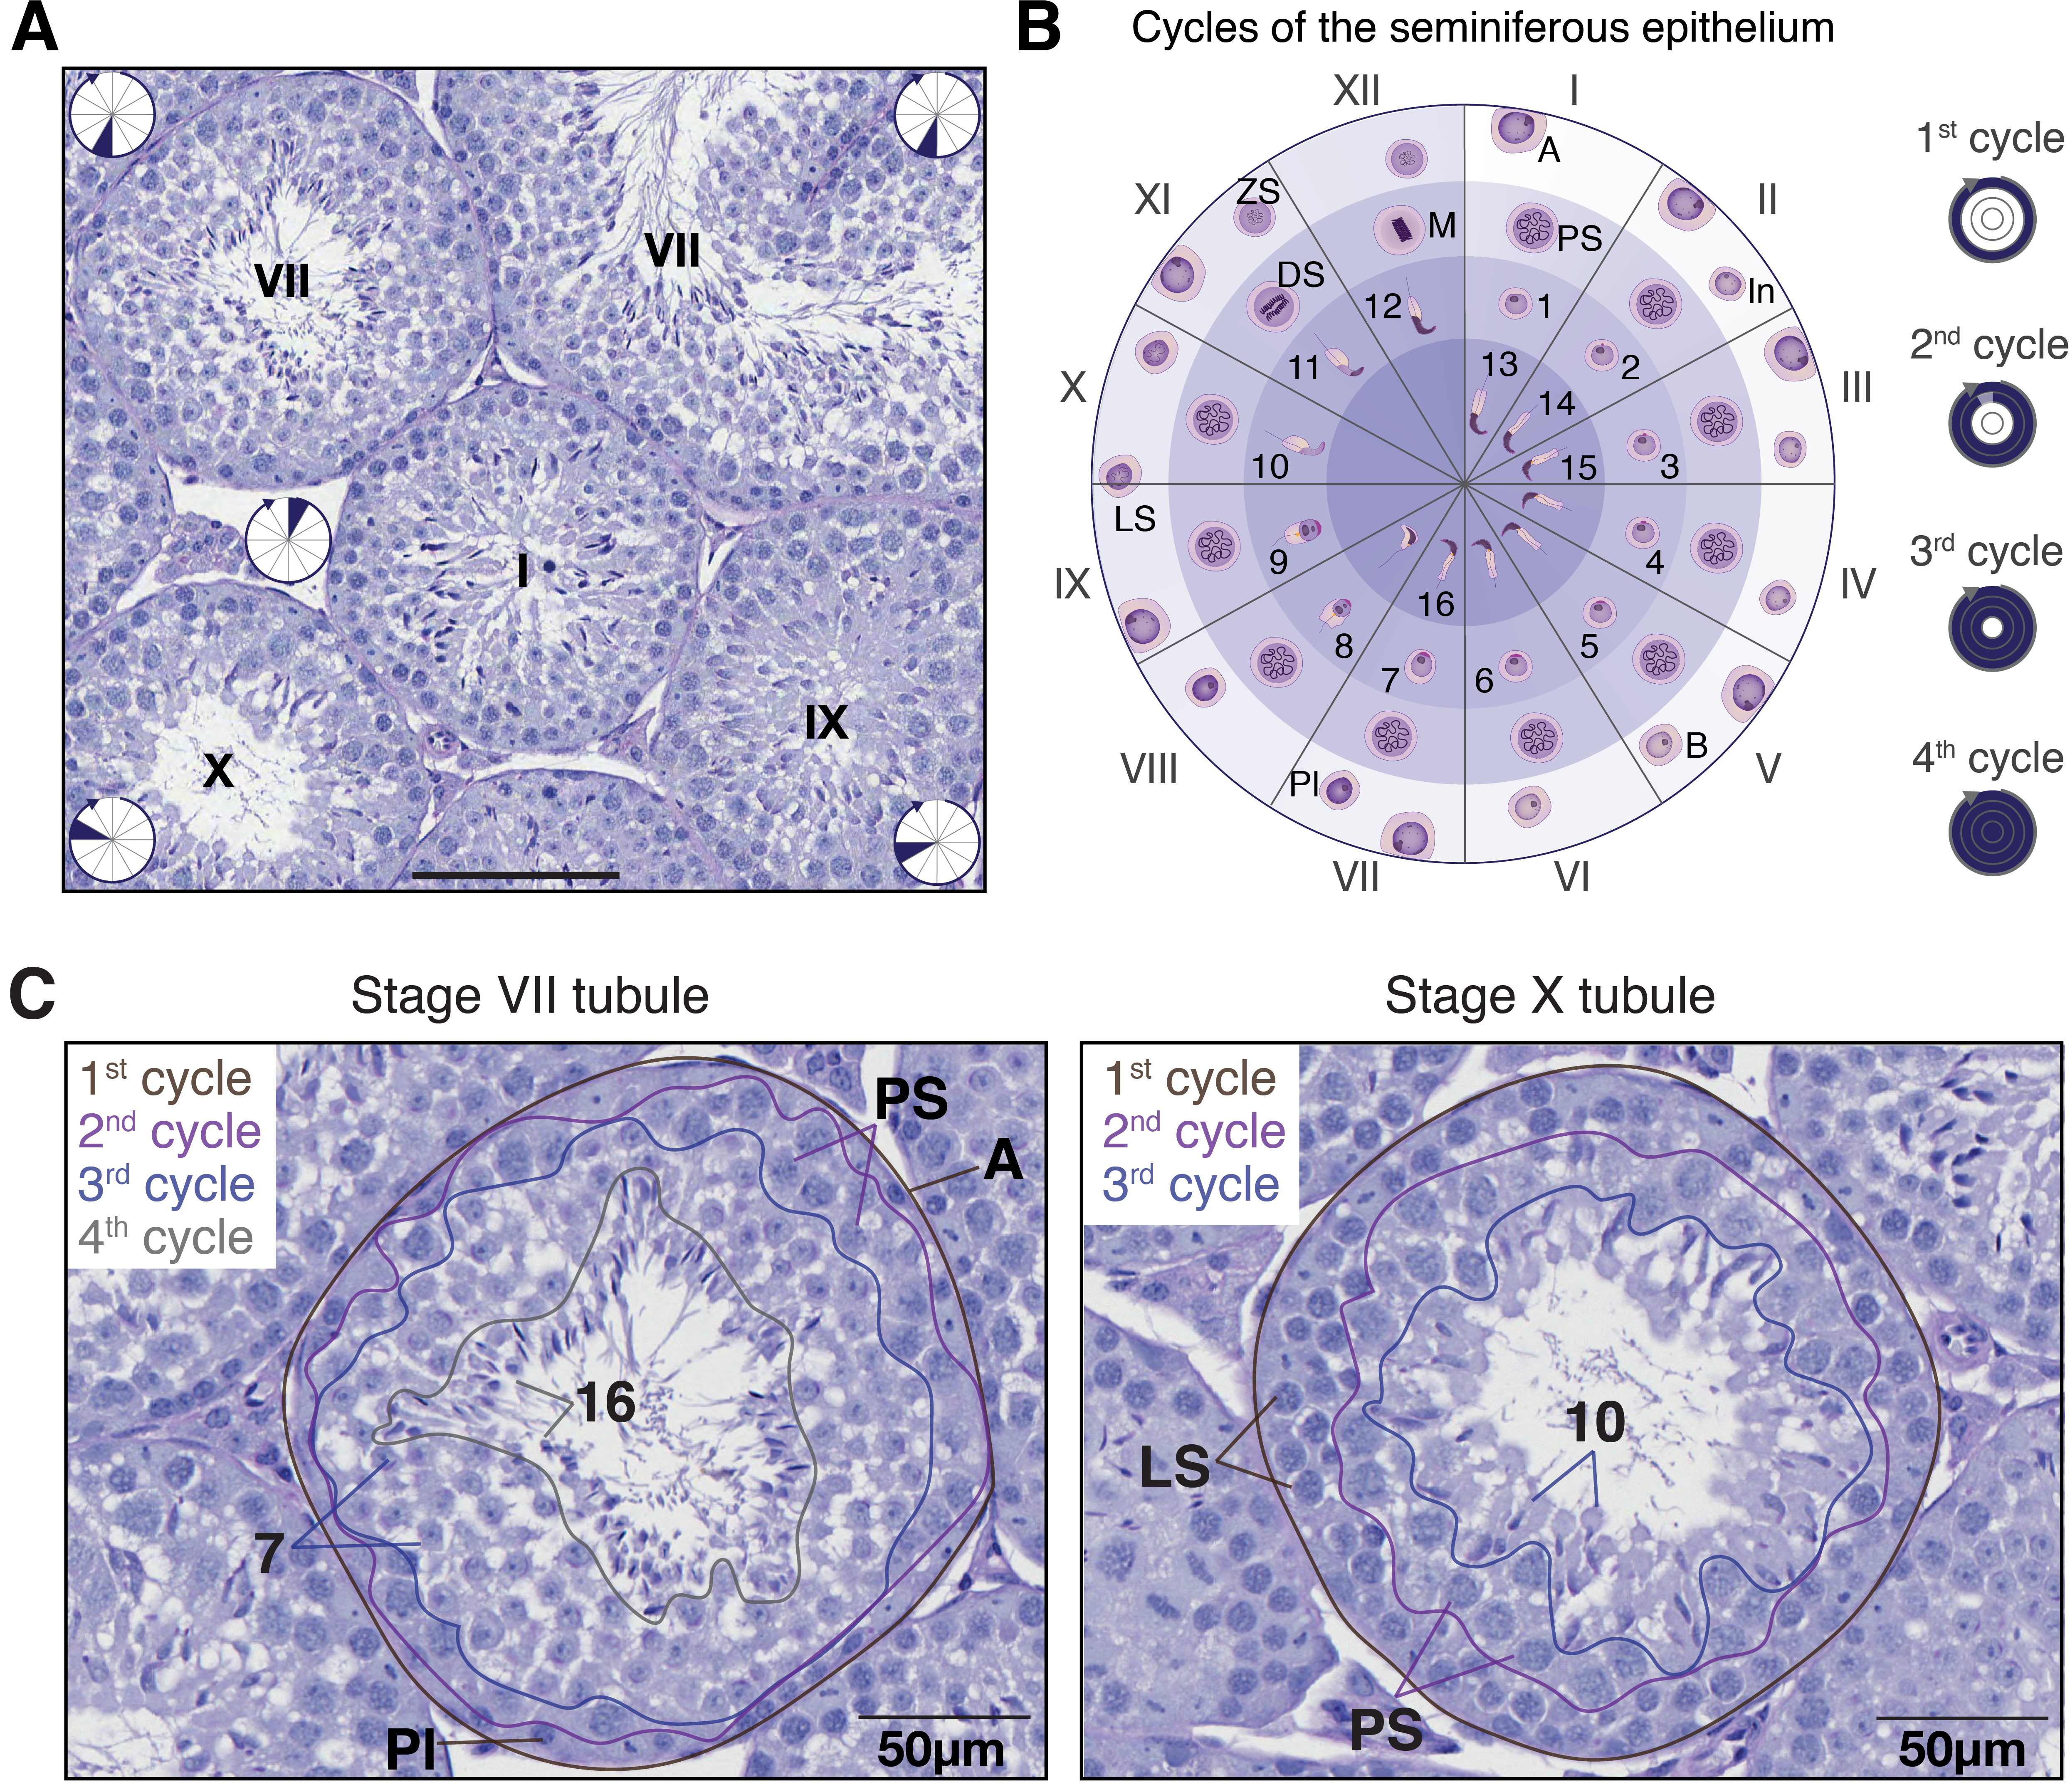
\includegraphics[width=0.48\textwidth]{Fig_1.png}
\caption[The scVI model.]{\textbf{The scVI model.} \\
Hierarchical representation of the scVI model. Shaded nodes indicate observed quantities. White nodes indicated latent random variables. Shaded diamonds represent constants which were set \emph{a priori}. White diamonds indicate variables shared across all genes and all cells. Edges show conditional dependency. Adapted from \citep{Lopez2018}.}
\label{fig0:scVI}
\vspace{-60mm}
\end{wrapfigure}

The latent representation is non-linearly transformed to generate a posterior distribution of model parameters based on a ZINB. For this, the transcript count $x_{n,g}$ of gene $g$ in cell $n$ is modelled as:\\

\begin{align*}
x_{n,g} & = 
 \left\lbrace
  \begin{aligned}
    & y_{n,g} && \textnormal{if} \; h_{n,g} = 0,  \\ 
    & 0 && \textnormal{otherwise}    	    
  \end{aligned}
\right.\\
h_{n,g} & \sim \textnormal{Bernoulli}(f_h^g(z_n,s_n))\\
y_{n,g} & \sim \textnormal{Poisson}(l_nw_{n.g})\\
w_{n,g} & \sim \textnormal{Gamma}(\rho^g_n, \theta)\\
\rho_n & = f_w(z_n,s_n)\\
l_n & \sim \textnormal{log-Normal}(l_{\mu},l^2_{\sigma})\\
z_n & \sim \textnormal{Normal}(0,I)
\end{align*}

\vspace{1cm}

In this model, the NB distribution is realized as a hierarchical formulation of $y_{n,g}$ being Poisson distributed around the latent random variable $l_n$ with an additional random effect $w_{n,g}$. Additionally, the zero-inflation of the model is controlled by the latent variable $h_{n,g}$. $l_n$ is a random variable that represents nuisance variation due to differences in capture efficiency and sequencing depth and correlates with log-library size. $l_n$ is log-normal distributed parametrized by $l_\mu,l_\sigma\in\mathbb{R}^B_+$ which are empirical mean and variance estimates of the log-library size per batch in $B$ and which are therefore constants in the model \textbf{(Fig.~\ref{fig0:scVI}A)}.\\

$w_{n,g}$ is Gamma distributed with the shape parameter $\rho_n^g$ and the scale parameter $\theta$. $\rho_g$ represents an intermediate matrix that relates the observations $x_{n,g}$ to the latent variables $z_n$. It provides a batch-corrected, normalized estimate of the percentage of transcripts in each cell $n$ from each gene $g$. $\theta$ is a global inverse-dispersion variable shared across all genes and all cells. The latent variable $z_n$ captures a latent representation of the data reflecting biological variation between the cells. $f_w$ and $f_h$ are neural networks mapping the latent space and batch annotation back to the full dimension of all genes: $\mathbb{R}^d\times{}\left\lbrace0,1\right\rbrace^B\rightarrow\mathbb{R}^G$.\\

Fast inference of this model is implemented via stochastic optimization. First, the latent variables $w_{n,g}$, $h_{n,g}$ and $y_{n,g}$ are integrated out by controlling that $p(x_{n,g}|z_n,l_n,s_n)$ has a closed form density and is ZINB (see Appendix A in \citep{Lopez2018}). In this formulation, the distribution of $x_{n,g}$ is only conditioned on the latent variables $z_n$ and $l_n$. The posterior distributions has therefore the following form: $p(z_n,l_n|x_{n,g},s_n)$. Mean-field variational inference is used to parametrised the posterior as:

\begin{equation}
p(z_n,l_n|x_{n,g},s_n)=p(z_n|x_{n,g},s_n)p(l_n|x_{n,g},s_n)
\end{equation} 

The variational distribution $q(z_n|\cdot)$ is chosen to be Gaussian with diagonal covariance matrix and mean and covariance are learned by a \gls{MLP} network similar to Kingma \emph{et al.}, 2013 \citep{Kingma2013}. Similarly, $q(l_n|\cdot)$ is chosen to be log-normal where the scalar mean and variance are learned by a MLP \citep{Kingma2013}. The authors used reparametrization to solve the variational lower bound of this system \cite{Lopez2018, Kingma2013}. Furthermore, scVI uses stochastic optimization by sampling 128 cells for optimizing the objective function. This approach is therefore fast (5 hours for > 1 million cells and 750 genes and 10 hours for > 1 million cells and 10,000 genes) and memory efficient. \\

The authors concluded that: 1. scRNA-Seq data is better fitted with a ZINB than log-Normal or zero-inflated log-Normal; 2. Zero-inflation is not needed as part of the model since the zeros in dataset can be explained by NB distribution; 3. When the number of cells is smaller than number of genes, scVI underfits the data \citep{Lopez2018}. The clear strength of the model is the fast estimation of model parameters that can be used for down-stream analysis (e.g. visualization, normalization, differential expression testing). The draw-back of this model is the inability to obtain gene-specific variability estimates but rather global variability measures calculated on the latent space. \\

As a future direction, generative models need to allow fast inference while providing interpretable model parameters that capture gene-specific measures of transcriptional noise. These measures should ideally be independent of technical noise, mean expression and possibly flexible enough to adjust for further confounding factors such as expression changes over a differentiation time-course. 
 

